\section{MAC network and our proposed simplification}

The MAC network~\cite{hudson2018compositional} is a recurrent model that performs
sequential reasoning, where each step involves analyzing a part of the question following 
which attention on the image is changed suitably.
At the end, a suitable answer is given based on this composite reasoning.
Both the question and image are transformed suitably prior to the reasoning process. 
For the question, a sequence of vectors obtained via word-embeddings is fed
to a bidirectional LSTM to produce a sequence of hidden state pairs. Each pair 
corresponds to a unique word in the question and denotes its 
\emph{contextual embedding}. The final states in each direction 
represent the \emph{global context} of that question.
Similarly each image is initially processed using a pre-trained network (using ResNet~\cite{he2016resnet}) to obtain a feature map. 
This is given as an input to a trainable neural network that consists of 
two CNN layers, resulting in a 3D tensor for each image in the data set. By viewing this
tensor a collection of 1D vectors in the last dimension, we call this
the \emph{knowledge base} of that image.

\begin{wrapfigure}{r}[5pt]{0.4\textwidth}
	\vspace{-15pt}
	\centering
	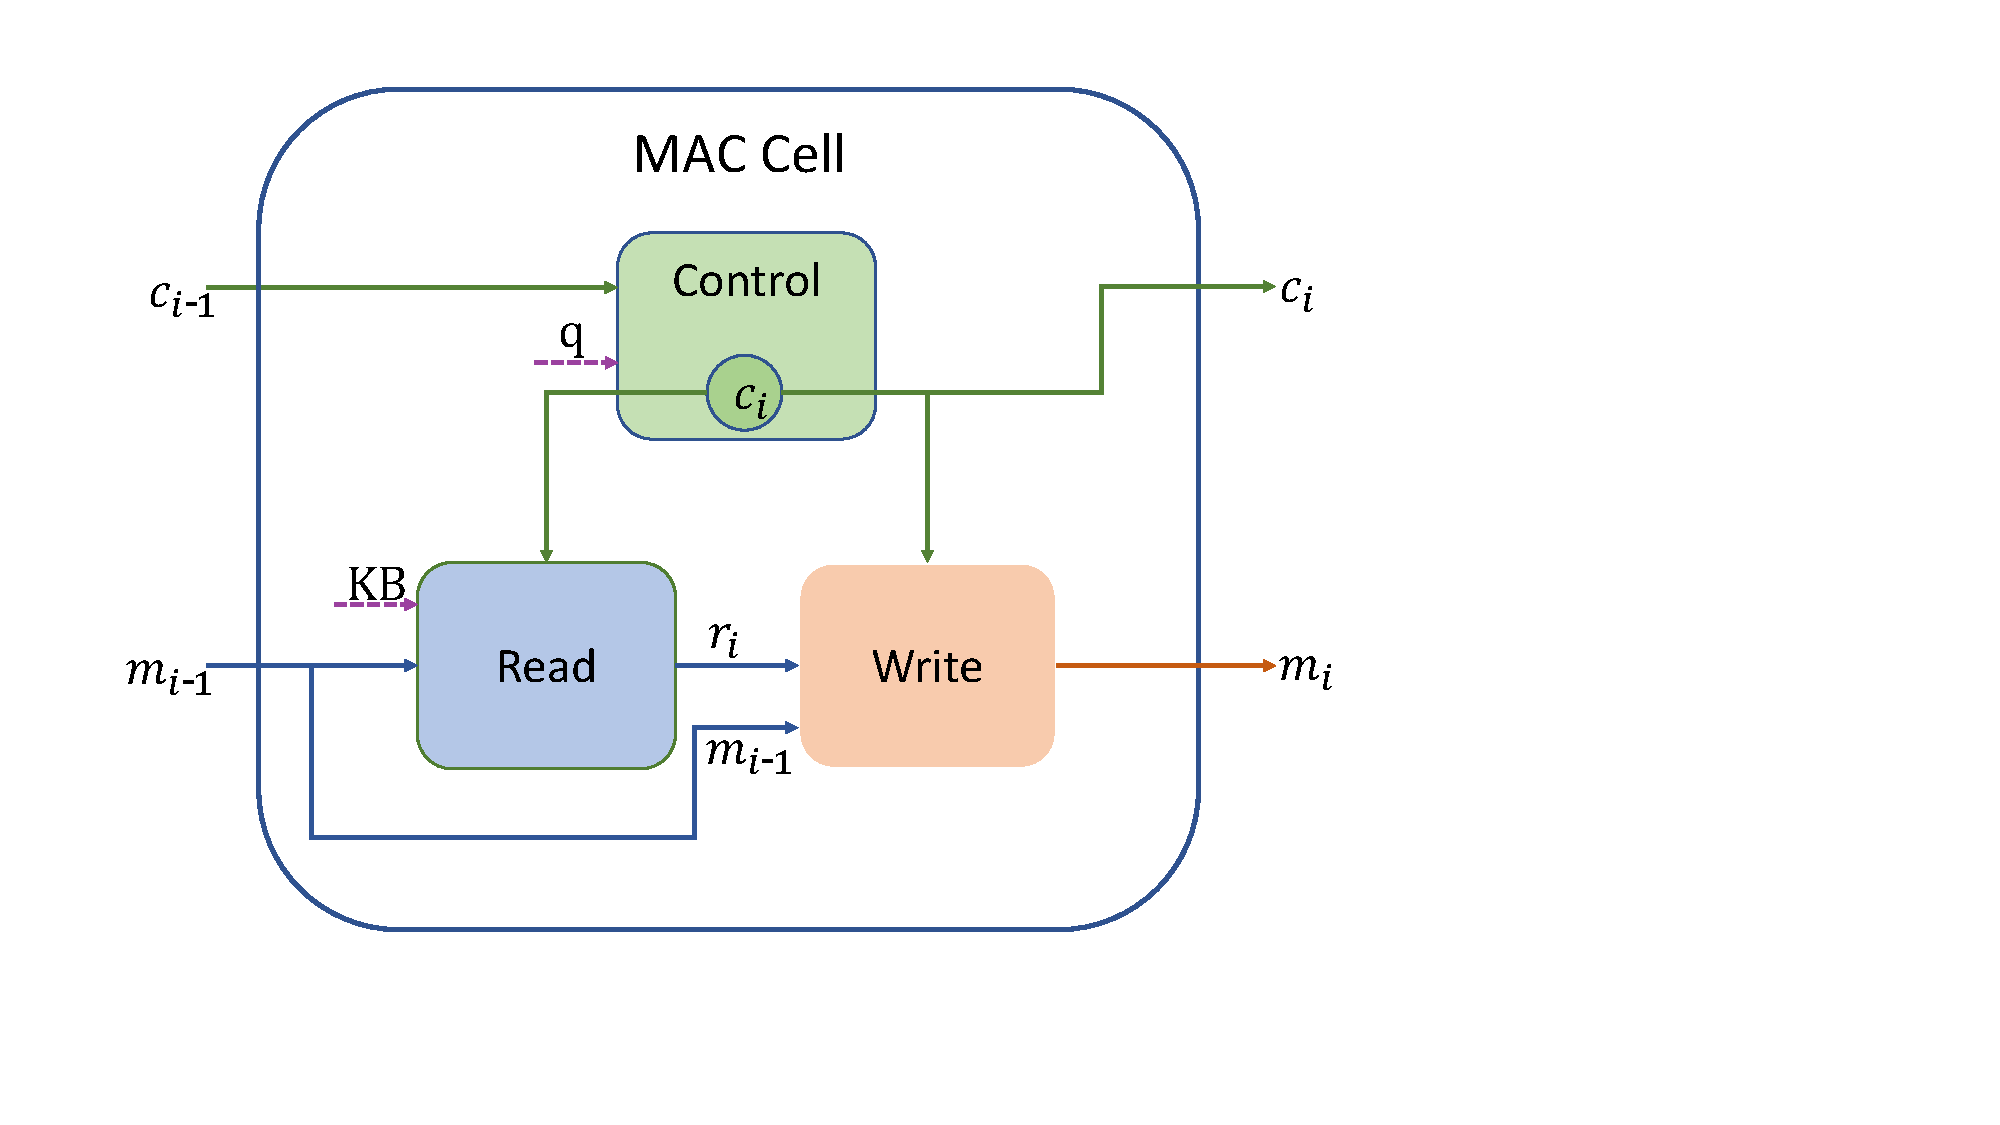
\includegraphics[width=\textwidth]{img/mac_cell.pdf}
	\caption{The MAC cell, reproduced on the basis of~\cite{hudson2018compositional}}
	\label{fig:mac_cell}
	\vspace{-5pt}
\end{wrapfigure}
	
The core of the network is a sequence of recurrent MAC cells, each performing one reasoning step (see Figure~\ref{fig:mac_cell}). At every step the network is driving the attention on one part of the question and the corresponding part of the image. This operation is made possible by the combination of 3 units working together: a control unit, a read unit and a write unit. The control unit is updating the control state and drives the attention over the question. Given this control state, the read unit then retrieves information from the memory and drives the attention over the image.
Finally, the write unit retrieves this visual information and updates the memory state.
The last part of the network is the output unit,  a simple classifier that process the concatenation of the global context  and the final memory state to produce a final answer.

By going through this recurrent process, the network performs a reasoning strategy that learns concepts and relations between them. MAC is performing state of the art accuracy on CLEVR and CLEVR Humans datasets.
In contrast to modular approaches \cite{andreas2016learning,hu2017learning,johnson2017inferring}, MAC is fully
differentiable and does not require additional supervision. It is making use of a single computational cell chained in sequence rather than a collection of custom modules deployed in a rigid tree structure.
In contrast to augmented CNN approaches, the MAC model provides an ability for relational reasoning with better generalization capacity, higher
computational efficiency and enhanced transparency \cite{hudson2018compositional}.

%\begin{figure}[htbp]
%	\centering
%	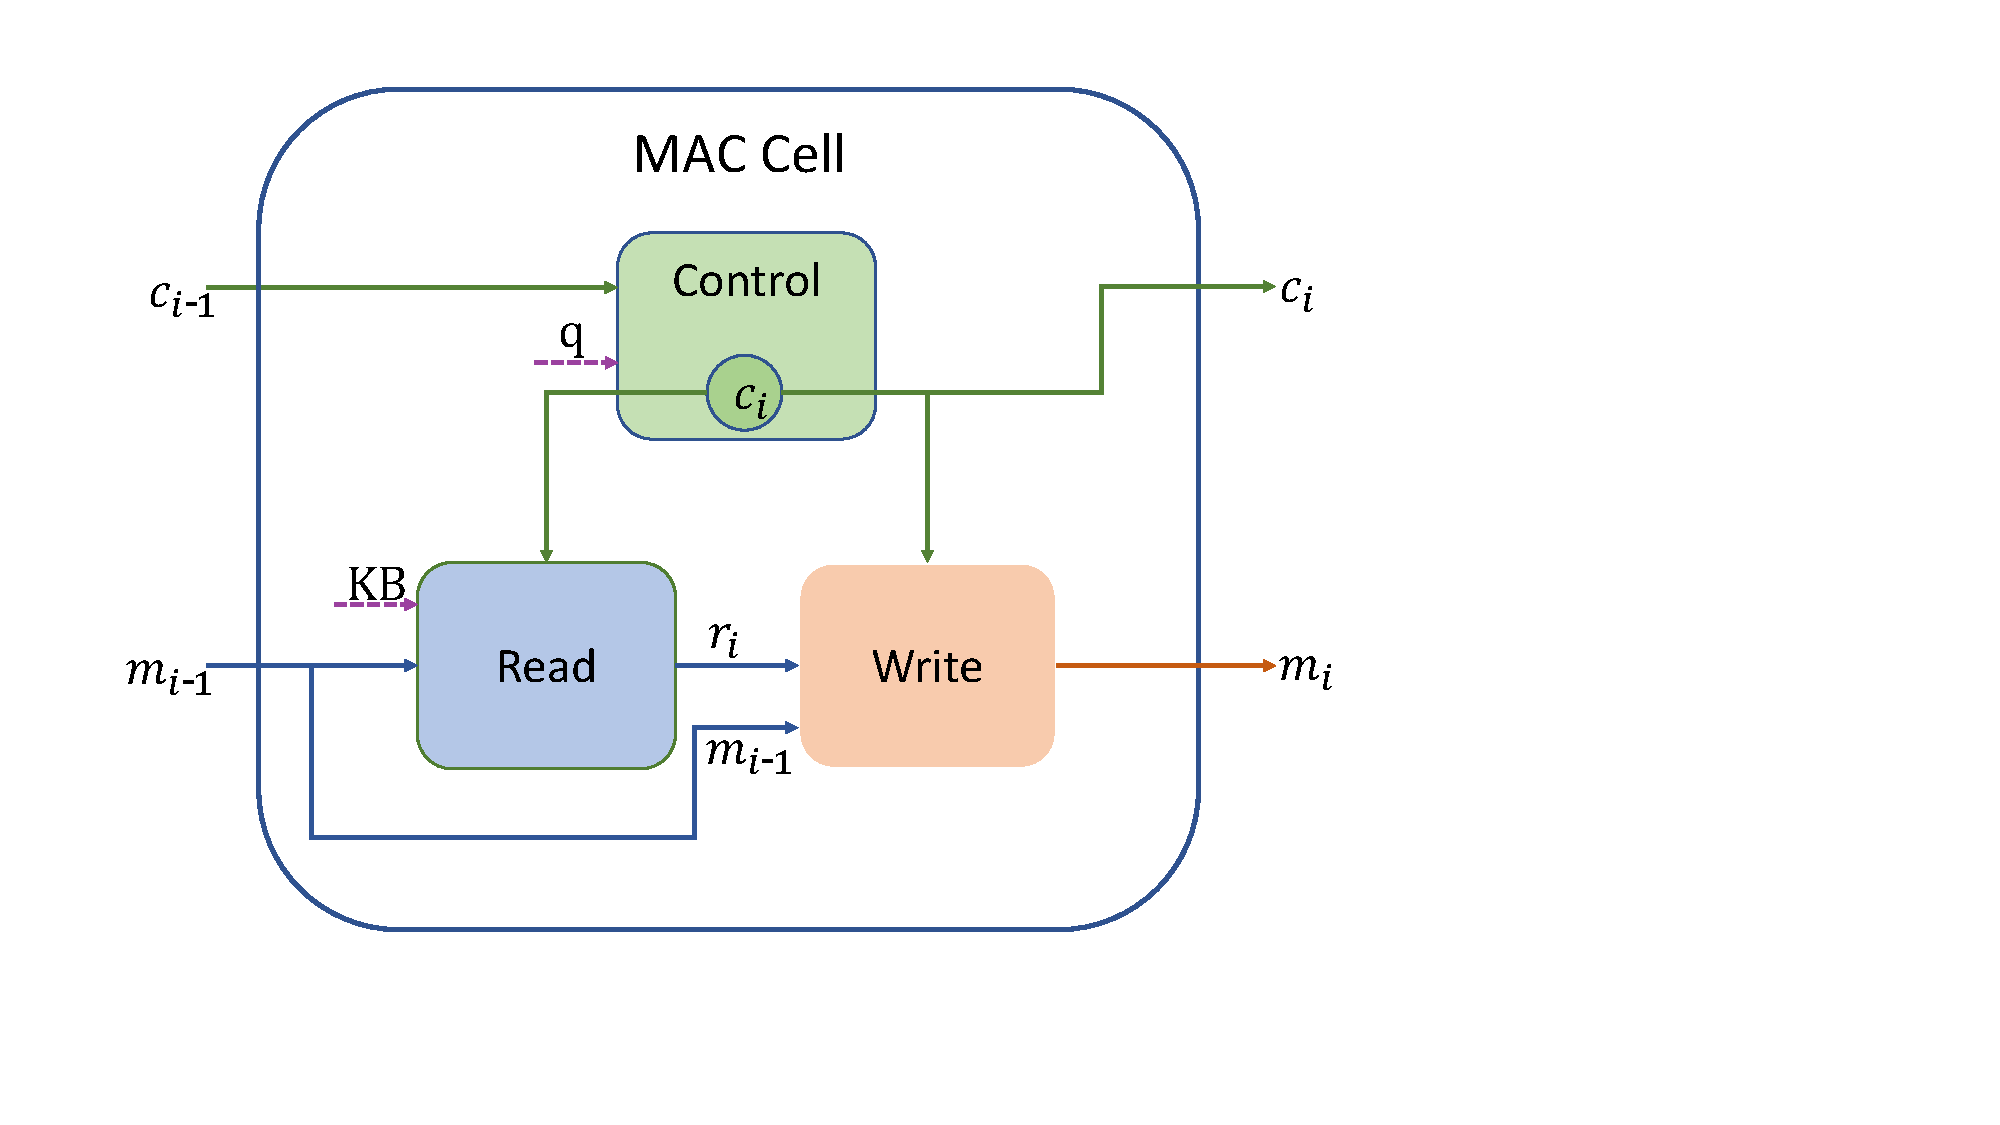
\includegraphics[width=0.4\textwidth]{img/mac_cell.pdf}
%	\caption{The MAC cell~\cite{hudsonManning18}}
%	\label{fig:mac_cell}
%\end{figure}
